\documentclass{standalone}
\usepackage{tikz}
\usepackage{pgfplots}
\pgfplotsset{width=32cm,height=18cm,compat=1.3}
\pgfplotsset{every tick label/.append style={font=\Huge}}
\usepackage{filecontents}

\usetikzlibrary{patterns}

\definecolor{citrine}{rgb}{0.89, 0.82, 0.04}

\begin{document}
	\centering
		\vspace{1.5em}
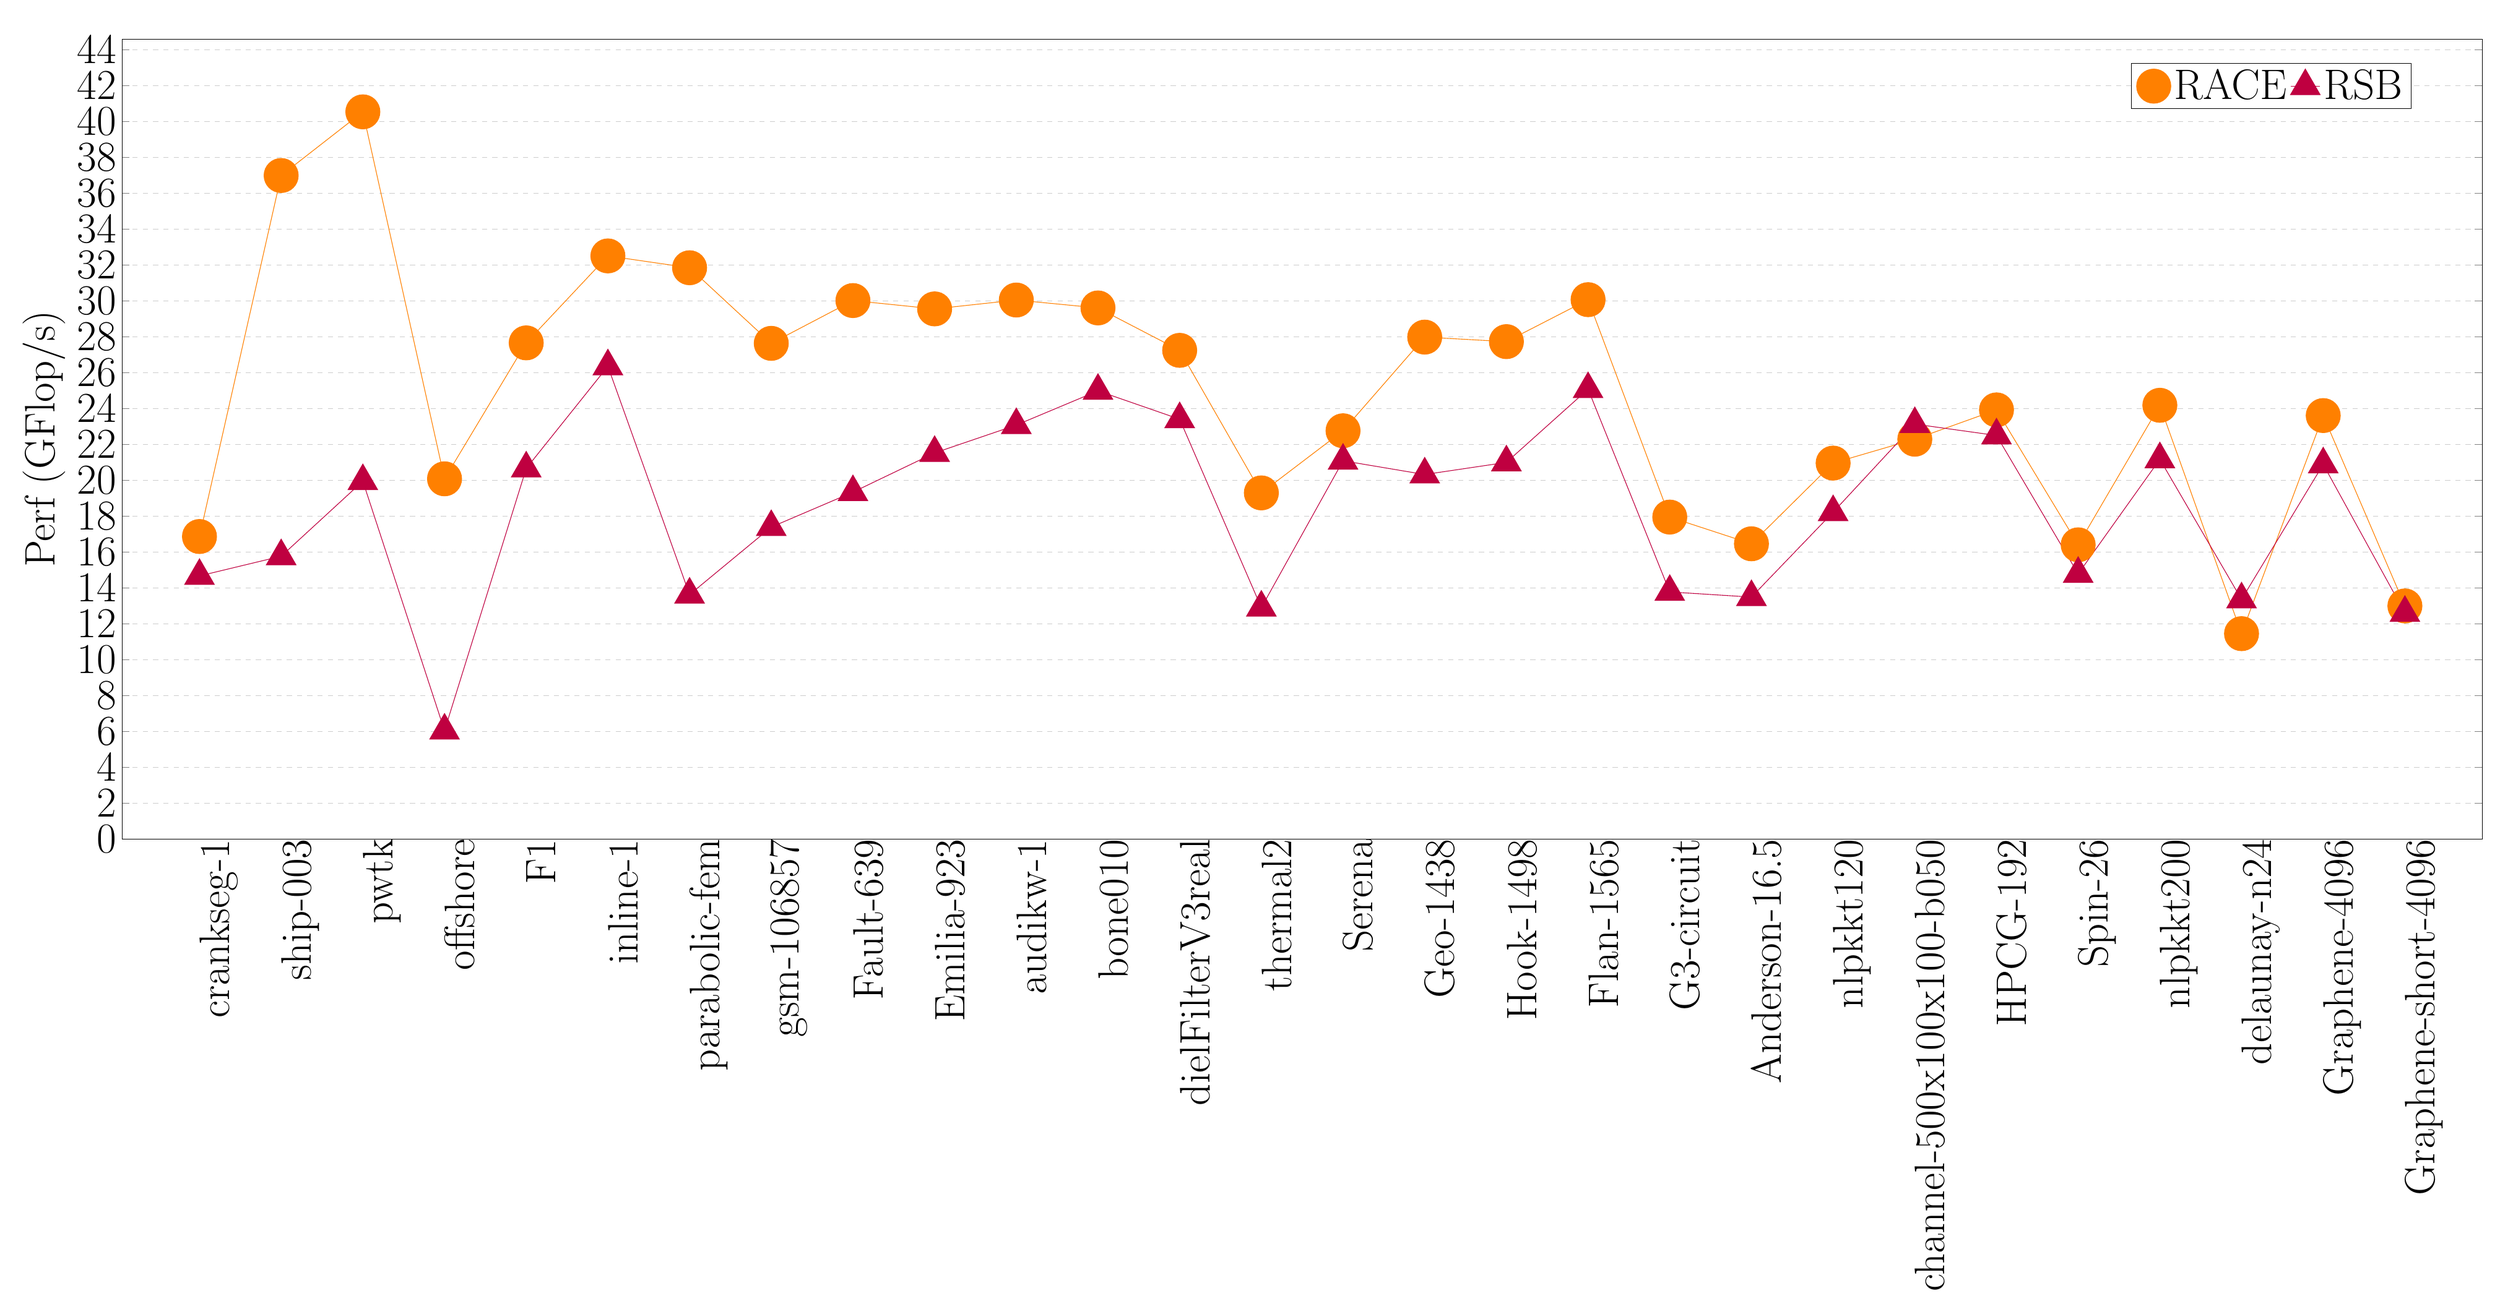
\begin{tikzpicture}
		%	\node at (13.25,15) {\LARGE{}};
			\begin{axis}[
		%	xmin=0.25, xmax=7.25,
			ymin=0, %ymax=3.25,
			xtick={1, 2, 3, 4, 5, 6, 7, 8, 9, 10, 11, 12, 13, 14, 15, 16, 17, 18, 19, 20, 21, 22, 23, 24, 25, 26, 27, 28},
		%	ytick={0,0.5,1,1.5,2,2.5,3},
			xticklabels={crankseg-1, ship-003, pwtk, offshore, F1, inline-1, parabolic-fem, gsm-106857, Fault-639, Emilia-923, audikw-1, bone010, dielFilterV3real, thermal2, Serena, Geo-1438, Hook-1498, Flan-1565, G3-circuit, Anderson-16.5, nlpkkt120, channel-500x100x100-b050, HPCG-192, Spin-26, nlpkkt200, delaunay-n24, Graphene-4096, Graphene-short-4096},
			width  = 50cm,
			height = 18cm,
			major x tick style = transparent,
			%	minor ytick={1, 5, 10, 15, 20, 25, 30 ,35,40},
			grid = minor,	
			%add_bar_commands
			ymajorgrids = true,
			grid style={dashed, gray!40},
			ylabel = {\Huge{Perf (GFlop/s)}},
		%	symbolic x coords={Graphene-2048-2048, Graphene-4096-4096, Spin-24-24-24},
			x tick label style={rotate=90, anchor=north east, inner sep=0mm, font={\Huge}},
			tick label style={font={\Huge}},
			scaled y ticks = false,
			enlarge x limits=0.035,
			legend cell align=left,
			legend style={font=\Huge},
			legend columns=-1,
			legend style={
				%at={(1,1.05)},
				%anchor=south east,
				%column sep=1ex,
				legend pos=north east
			},
			%spl_legend_code
			title= {\Huge\scalebox{1.5}{{}}}
			]

\addplot[mark=*, mark size=10pt, mark options={orange}, draw=orange ] plot coordinates{(1,16.854992) (2,36.979831) (3,40.528888) (4,20.072225) (5,27.650065) (6,32.497825) (7,31.837543) (8,27.622948) (9,30.008732) (10,29.544466) (11,30.038410) (12,29.598056) (13,27.233392) (14,19.287252) (15,22.750551) (16,27.971316) (17,27.719366) (18,30.058614) (19,17.938689) (20,16.449635) (21,20.948219) (22,22.279768) (23,23.914583) (24,16.392259) (25,24.170988) (26,11.440436) (27,23.598034) (28,12.986649)};
\addplot[mark=triangle*, mark size=10pt, mark options={purple}, draw=purple ] plot coordinates{(1,14.659662) (2,15.755979) (3,19.940788) (4,6.035534) (5,20.649774) (6,26.343394) (7,13.616971) (8,17.381188) (9,19.328295) (10,21.514780) (11,23.067242) (12,24.976454) (13,23.396038) (14,12.891779) (15,21.077145) (16,20.312141) (17,20.986794) (18,25.069384) (19,13.767292) (20,13.478755) (21,18.211690) (22,23.121443) (23,22.488479) (24,14.773625) (25,21.161154) (26,13.349274) (27,20.876893) (28,12.596639)};
	%addplot cmd

	\legend{RACE, RSB}

	\end{axis}			
\end{tikzpicture}

\end{document}

